\documentclass[11pt,a4paper]{article}
\usepackage{graphicx}
%\usepackage{isabelle,isabellesym}

\usepackage{proof}

%\usepackage{isabelle}

%\usepackage[isasymonly]{hol-ocl-isar}
\usepackage{hol-ocl-isar}

\usepackage{amsmath}
\usepackage{amssymb}

% this should be the last package used
\usepackage{pdfsetup}

% way no ... bu
\usepackage[draft]{fixme}

% urls in roman style, theory text in math-similar italics
\urlstyle{rm}
%\isabellestyle{it}

\newcommand{\bgtt}{\bgroup\isabellestyle{default}\isabellestyle{tt}\isastyle%
\renewcommand{\isadigit}[1]{##1}}
\newcommand{\entt}{\egroup}

%\renewenvironment{isatagML}{\bgtt}{\entt}
%\isadroptag{ML}

\newcommand{\isasymboxplus}{\isamath{\boxplus}}
\newcommand{\isactrlcircusaction}{}
\newcommand{\isactrlbegincircusschema}{}
\newcommand{\isactrlendcircusschema}{}

\newcommand{\ie}{\textit{i.e.}\ }
\newcommand{\eg}{\textit{e.g.}\ }
\newcommand{\wrt}{\textit{w.r.t.}\ }

\usepackage{listings}
\usepackage{lstisar-mbt}

\usepackage{multicol}

\usepackage[color]{circus}

\begin{document}

\title{Isabelle/Circus}
\author{Abderrahmane Feliachi, Marie-Claude Gaudel, Makarius Wenzel \\
        and Burkhart Wolff}
\maketitle

\begin{abstract}
The Circus specification language combines elements for complex data and behavior specifications, 
using an integration of Z and CSP with a refinement calculus. Its semantics is based on Hoare and He's
unifying theories of programming (UTP).

Isabelle/Circus is a formalization of the UTP and the Circus language in Isabelle/HOL.
It contains proof rules and tactic support that allows for proofs
of refinement for Circus processes (involving both data and behavioral aspects).

This environment supports a syntax for the semantic definitions which is close to textbook presentations of Circus.

These theories are presented with details in \cite{fgw11rapport-lri}. This document is a technical appendix of this report.
\end{abstract}

\tableofcontents

\begin{center}
  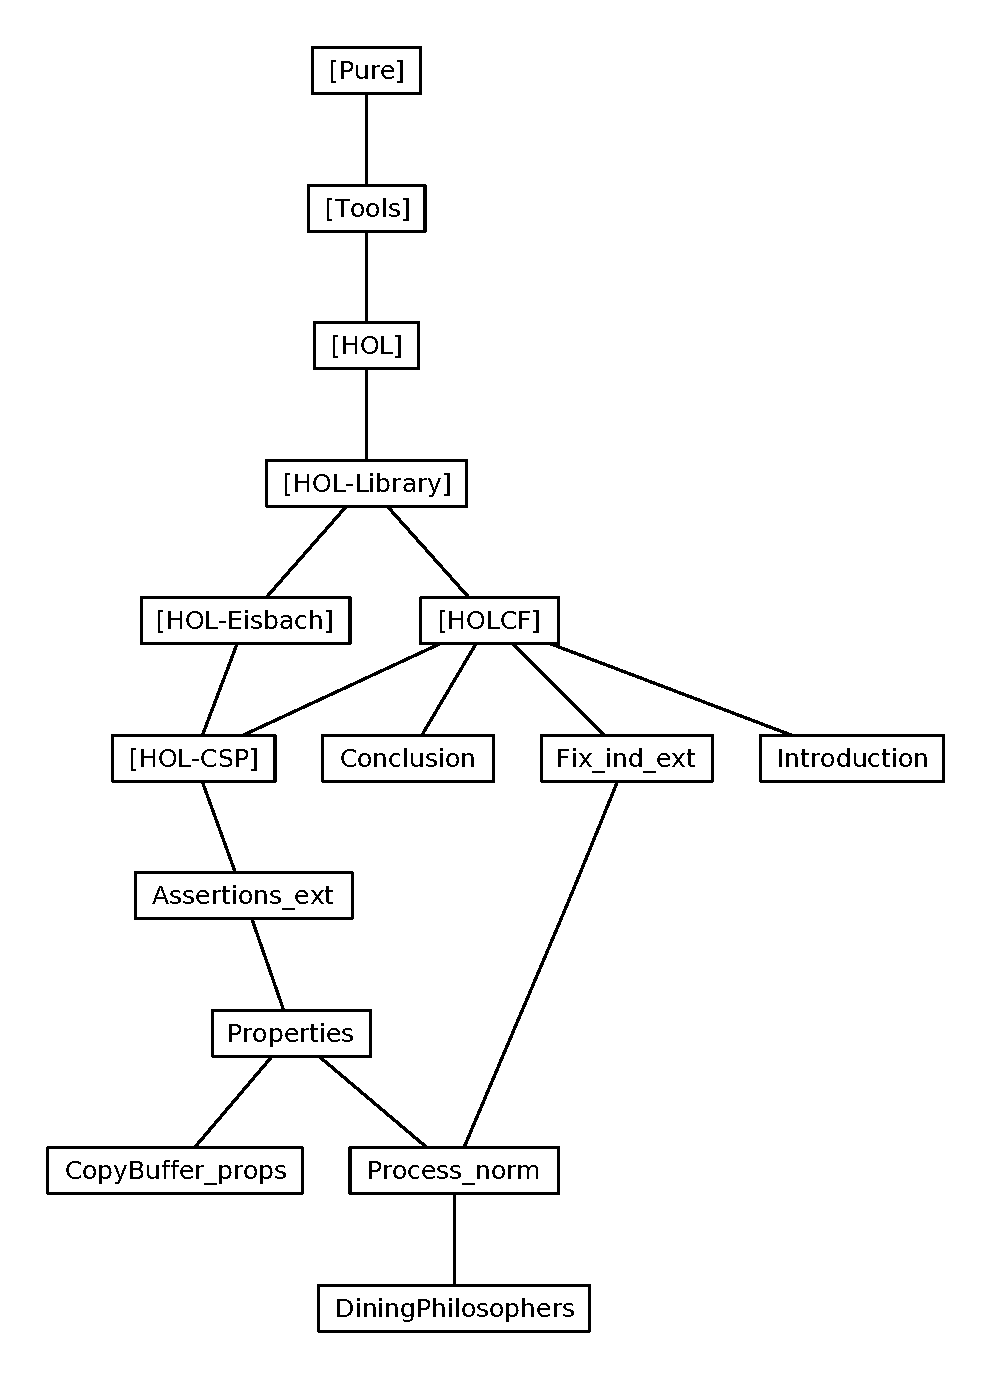
\includegraphics[width=\textwidth,height=\textheight,keepaspectratio]{session_graph}
\end{center}

\newpage

\section{Introduction} 
Many systems involve both complex (sometimes infinite) data structures and interactions between concurrent processes. Refinement of abstract specifications of such systems into more concrete ones, requires an appropriate formalisation of 
refinement and appropriate proof support.


There are several combinations of process-oriented modeling languages
with data-oriented specification formalisms such as Z or B or CASL; examples
are discussed in \cite{Butler99csp2b:a,Fischer:1998:CZP:647283.722938,Taguchi:1997:SCS:523981.852142,Roggenbach:2006}.
In this paper, we consider \Circus\ \cite{WC02}, a
language for refinement, that supports modeling of high-level
specifications, designs, and concrete programs. It is representative
of a class of languages that provide facilities to model data types,
using a predicate-based notation, and patterns of interactions, without imposing 
architectural restrictions. It is this feature that makes
it suitable for reasoning about both abstract and low-level
designs. 

We present a ``shallow embedding'' of the \Circus\
semantics enabling state variables and channels in \Circus\ to have
arbitrary HOL types. Therefore, the entire handling of typing can be
completely shifted to the (efficiently implemented) Isabelle
type-checker and is therefore implicit in proofs. This drastically
simplifies definitions and proofs, and makes the reuse of
standardized proof procedures possible. Compared to implementations
based on a ``deep embedding'' such as \cite{ZC09} this significantly improves the
usability of the resulting proof environment.

Our representation brings particular technical challenges and contributions concerning
some important notions about variables. The main challenge was to represent alphabets 
and bindings in a typed way that preserves the semantics and improves deduction. 
We provide 
a representation of bindings without an explicit management of alphabets. 
However, the 
representation of some core concepts in the
unifying theories of programming (UTP) and \Circus\ constructs (variable scopes and renaming) became 
challenging. 
Thus, we propose a (stack-based) solution that allows the coding of state variables 
scoping with no need for renaming. This solution is even a contribution to the UTP theory that 
does not allow nested variable scoping. Some challenging and tricky definitions (e.g. channels 
and name sets) are explained in this paper.

This paper is organized as follows. The next section gives an introduction to the basics of our 
work: Isabelle/HOL, UTP and \Circus\ with a short example of a \Circus\ process. In Section \ref{Section:CircusHOL}, 
we present our embedding of the basic concepts of  \Circus\  (alphabet, variables ...). We introduce the representation of  some \Circus\ actions and process, with an overview of the Isabelle/\Circus\ syntax. In 
Section \ref{Section:framework}, we show on an example, how  Isabelle/\Circus\  can be used to write specifications. 
We give some details on what %the system 
is happening ``behind the scenes'' when the system parses each part of the specification. In the last part of 
this section, we show how to write proofs based on specifications, and give a refinement proof example.
A more developed version of this paper can be found in \cite{fgw11rapport-lri}.
 

\section{Background}
\label{Section:background}

\subsection{Isabelle, HOL and Isabelle/HOL}
\label{IsaHOL}
\subsubsection{isar} \cite{nipkow.ea:isabelle:2002} is a generic theorem prover
implemented in SML.  It is based on the so-called ``LCF-style
architecture'', which makes it possible to extend a small trusted logical
kernel by user-programmed procedures in a logically safe way. New
object logics can be introduced to Isabelle by specifying their syntax
and semantics, by deriving its inference rules from there and program specific
tactic support for the object logic. Isabelle is based on a typed $\lambda$-calculus
including a Haskell-style type-system with type-classes 
(e.g. in $\alpha::\text{order}$, the type-variable ranges over all types
that posses a partial ordering.)

\subsubsection{Higher-order logic (HOL)}~\cite{church:types:1940,andrews:introduction:2002} is a
classical logic based on a simple type system.  It provides the usual
logical connectives like $\_ \land \_$, $\_ \implies\_$, $\lnot \_ $
as well as the object-logical quantifiers $\forall x\spot P\ x$ and
$\exists x\spot P\ x$; in contrast to first-order logic, quantifiers
may range over arbitrary types, including total functions
$f :: \alpha \Rightarrow \beta$. HOL is centered around
extensional equality $\_ = \_ :: \alpha \Rightarrow \alpha
\Rightarrow \text{bool}$.  HOL is more expressive than first-order
logic, since, \eg, induction schemes can be expressed inside the
logic. Being based on some polymorphically typed $\lambda$-calculus,
HOL can be viewed as a combination of a programming language
like SML or Haskell and a specification language providing
powerful logical quantifiers ranging over elementary and function
types.

\subsubsection{Isabelle/HOL} is an instance of Isabelle with higher-order 
logic. It provides a rich collection of library theories like sets, pairs,
relations, partial functions lists, multi-sets, orderings, and various
arithmetic theories which only contain rules derived from conservative, \ie 
logically safe definitions.  Setups for the automated proof procedures like
\inlineisar{simp}, \inlineisar{auto}, and arithmetic types such as \inlineisar{int} are provided.

\subsection{Advanced Specification Constructs in Isabelle/HOL}
\label{Subsection:advconstructs}
\subsubsection{Constant definitions.} In its easiest form, constant definitions
are definitional logical axioms of the form $c \equiv E$ where c is a fresh
constant symbol not occurring in $E$ which is closed (both wrt. variables
and type variables). For example:
\begin{isar}
definition upd::(\<alpha>\<Rightarrow>\<beta>)\<Rightarrow>\<alpha>\<Rightarrow>\<beta>\<Rightarrow>(\<alpha>\<Rightarrow>\<beta>)         ("_(|_ := _|)")
where       "upd f x v \<equiv>   \<lambda> z. if x=z then v else f z"
\end{isar}
The pragma \inlineisar+("_(| _ := _|)")+ for the Isabelle syntax engine introduces the
notation \inlineisar+f(|x:=y|)+ for \inlineisar+upd f x y+.
Moreover, some elaborate preprocessing allows for recursive
definitions, provided that a termination ordering can be established. Such recursive 
definitions are thus internally reduced to definitional axioms.

\subsubsection{Type definitions.} Types can be introduced in Isabelle/HOL 
in different ways. 
The most general way to safely introduce new types is 
 using the \inlineisar+typedef+ construct. This allows 
introducing a type as a non-empty subset of an existing type. More
precisely, the new type is specified to be isomorphic to this
non-empty subset. For instance:
\begin{isar}
 typedef mytype = "{x::nat. x < 10}"
\end{isar}
This definition requires that the set is non-empty:
\inlineisar+\<exists>x. x\<in>{x::nat. x<10}+, which is 
easy to prove in this case:
\begin{isar}
 by (rule_tac x = 1 in exI, simp)
\end{isar}
where \inlineisar+rule_tac+ is a tactic that applies an introduction rule, and \inlineisar+exI+ corresponds to the introduction of the existential quantification.


Similarly, the \inlineisar+datatype+ command allows the definition of
inductive datatypes. It introduces a datatype using a list
of \emph{constructors}. For instance, a logical compiler is invoked for the
following introduction of the type \inlineisar+option+:
\begin{isar}
 datatype \<alpha>  option   = None | Some \<alpha>
\end{isar}
which generates the underlying type definition and derives distinctness rules and induction
principles. Besides the \emph{constructors}
\inlineisar+None+ and \inlineisar+Some+, the following match-operator and his rules are also generated:

$\HolCase\ap x\ap\HolOf~\HolNone \isasymRightarrow ...\ap \mid \HolSome{a} \isasymRightarrow ...$ 

\subsubsection{Extensible records.}
Isabelle/HOL's support for \emph{extensible records} is of particular importance 
for our work.
Record types are denoted, for example, by:
\begin{isar}
 record T =  a::T_1 
             b::T_2 
\end{isar}
which implicitly introduces the record constructor \inlineisar+(|a:=e_1,b:=e_2|)+ 
and the update of record r in field a, written as \inlineisar+r(|a:= x|)+. 
Extensible records are represented internally by cartesian products with an 
implicit free component $\delta$, i.e. in this case by a triple of the type 
\inlineisar+T_1 \<times> T_2 \<times> \<delta>+. The third component can be referenced
by a \emph{special selector}   \inlineisar+more+ available on extensible records.
Thus, the record \inlineisar+T+ can be
extended later on using the syntax: 
\begin{isar}
 record ET =  T +  c::T_3 
\end{isar}
The key point is that theorems can be established, once and for all,
on \inlineisar+T+ types, even if future parts of the record are not
yet known, and reused in the later definition and proofs over
\inlineisar+ET+-values. 
Using this feature, we can model the effect of defining the
alphabet of UTP processes incrementally while maintaining 
the full expressivity of HOL wrt. the types of 
\inlineisar+T_1+, \inlineisar+T_2+ and \inlineisar+T_3+.

\subsection{\Circus\  and its UTP Foundation}
\label{CircusUTP}
\Circus\ is a formal specification language \cite{WC02} which
integrates the notions of states and complex data types (in a Z-like
style) and communicating parallel processes inspired from CSP.
From Z, the language inherits the notion of a schema used to
model sets of (ground) states as well as syntactic machinery to describe
pre-states and post-states; from CSP, the language inherits 
the concept of \emph{communication events} and typed communication channels, 
the concepts of deterministic and non-deterministic choice
(reflected by the process combinators $P~\square~P'$ and $P~\sqcap~P'$),
the concept of concealment (hiding) $P \backslash A$ of events in $A$ occurring in 
in the evolution of process $P$.
Due to the presence of state variables, the \Circus\  synchronous communication operator syntax is slightly different frome CSP:  $P\ \llbracket\ n \ |\ c\ |\ n'\ \rrbracket P'$ means that $P$ and
$P'$ communicate via the channels mentioned in $c$; moreover, $P$ may modify the variables mentioned in $n$ only, and $P'$ in $n'$ only, $n$ and $n'$ are disjoint name sets.

Moreover, the language comes with a formal notion of refinement based on a 
denotational semantics. It follows the failure/divergence semantics \cite{Roscoe:1997:TPC:550448}, 
(but coined in terms of the UTP \cite{CircusDS}) providing a notion of execution trace \inlineisar+tr+, 
refusals \inlineisar+ref+, and divergences. %(see below)).
It is expressed in terms of the UTP \cite{HJ98} 
which makes it amenable to other refinement-notions in UTP. %The semantics allows 
Figure \ref{figure:Fig} presents a simple \Circus\ specification,  \inlineisar+FIG+, the fresh identifiers generator.\\

\vspace{-.8cm}
\begin{figure}[h]
\begin{zed}
    [ID]
\end{zed}
\vspace{-.8cm}
\begin{circus}
    \circchannel\ req\\
    \circchannel\ ret, out: ID
\end{circus}
\vspace{-.9cm}
\begin{circus}
    \circprocess\ FIG ~~\circdef~~ \circbegin\
\end{circus}
\vspace{-1.0cm}
\begin{circusaction}
     \circstate\ S ~~==~~ [~ idS: \power~ID  ~]   
 \end{circusaction}
\vspace{-1.0cm}
 \begin{circusaction}
     Init ~~\circdef~~ idS := \emptyset
 \end{circusaction}%
\vspace{-1.2cm}
\begin{multicols}{2}
\begin{schema}{Out}
     \Delta S \\
      v!: ID
 \where
    v! \notin idS \\ 
    idS' = idS \cup \{ v! \}
 \end{schema}%
\begin{schema}{Remove}
     \Delta S \\
      x?: ID
 \where
     idS' = idS \setminus \{ x? \}
 \end{schema}%
\end{multicols}
\vspace{-.5cm}
 \begin{circusaction}
     \circspot\ Init \circseq\ \circvar\ v : ID \circspot\ \\
  (\circmu\ X \circspot\ (req \then Out \circseq\ out!v \then \Skip\ \extchoice\ ret?x \then Remove)\circseq\ X)
 \end{circusaction}
\vspace{-.9cm}
 \begin{circus}
     \circend\
 \end{circus}
\vspace{-1cm}
\caption{\label{figure:Fig} The Fresh Identifiers Generator in (Textbook) \Circus\ }
\vspace{-.55cm}
\end{figure}

\subsubsection{Predicates and Relations.}
The UTP is a semantic framework based on an alphabetized relational
calculus. An \emph{alphabetized predicate} is a pair ($alphabet$,
$predicate$) where the free variables appearing in the predicate are
all in the alphabet, e.g. $(\{x, y\}, x > y)$. As such, it is very similar to
the concept of a \emph{schema} in Z. In the base theory Isabelle/UTP
of this work, we represent alphabetized predicates  by sets of (extensible) 
records, e.g.  \inlineisar+{A. x A > y A}+. 

An \emph{alphabetized relation} is an alphabetized predicate where the
alphabet is composed of input (undecorated) and output (dashed)
variables. In this case the predicate describes a relation between
input and output variables, for example $(\{x, x', y, y'\}, x' = x + y)$
which is a notation for: \inlineisar*{(A,A').x A' = x A + y A}*, which is
a set of pairs, thus a relation. 

Standard predicate calculus operators are used to combine alphabetized
predicates. The definition of these operators is very similar to the
standard one, with some additional constraints on the alphabets.

\subsubsection{Designs and processes.}
\label{sec:design-and-processes}
In UTP, in order to explicitly record the termination of a program, a subset
of alphabetized relations is introduced. These relations are called
$designs$ and their alphabet should contain the special boolean
observational variable \inlineisar+ok+. 
% This variable 
It is used to record the start and termination of a program. A UTP design is defined as follows
in Isabelle:
\begin{isar}
    (P \<turnstile> Q) \<equiv>  \<lambda> (A,A'). (ok A \<and>   P (A,A')) \<longrightarrow>  (ok A' \<and>  Q (A,A')) 
\end{isar}
Following the way of UTP to describe reactive processes,
% we need to add 
more observational variables are needed to record the interaction %of these processes 
with the environment. Three observational variables are defined for this subset
of relations: \inlineisar+wait+, \inlineisar+tr+ and \inlineisar+ref+. The boolean variable \inlineisar+wait+
records if the process is waiting for an interaction or has
terminated. \inlineisar+tr+ records the list (trace) of interactions
the process has performed so far. The variable \inlineisar+ref+ contains the set
of interactions (events) the process may refuse to perform. These observational variables defines the basic alphabet of all reactive processes called ``\inlineisar+alpha_rp+''.

Some healthiness conditions are defined over \inlineisar+wait+, \inlineisar+tr+ and \inlineisar+ref+ to 
ensure that a recative process satisfies some properties \cite{CW06} (see Table 2 in \cite{fgw11rapport-lri}).

A CSP process is a UTP reactive process that satisfies two additional
healthiness conditions% called $CSP1$ and $CSP2$ 
(all well-formedness conditions 
can be found in \cite{fgw11rapport-lri}). 
A process that satisfies these conditions is said to be CSP healthy.

\section{Isabelle/\Circus } 
\label{Section:CircusHOL}

\begin{figure}[h]
\vspace{-0.6 cm}
\begin{minipage}{5cm}
$
  \begin{array}{lcl}
    % ----------------------------------------------------------------%
    \mathsf{Process} & %
    \mathsf{::=} & \mathsf{\textbf{circusprocess}\ Tpar^*\ name\ \textbf{=}\ PParagraph^*\ \textbf{where}\  Action} \
    \\ %
    \mathsf{PParagraph} & %
    \mathsf{::=} & \mathsf{AlphabetP }\ \mathsf{|}\ \mathsf{StateP }\ \mathsf{|}\ \mathsf{ ChannelP }\ \mathsf{|}\ \mathsf{ NamesetP }\ \mathsf{|}\ \mathsf{ ChansetP }\ \mathsf{|}\ \mathsf{ SchemaP }\ \\%
& \mathsf{|}\ & \mathsf{ ActionP} \
    \\ %
    \mathsf{AlphabetP} & %
    \mathsf{::=} & \mathsf{\textbf{alphabet}\ \textbf{[ }\ vardecl^+\  \textbf{] }} \
    \\ %
    \mathsf{vardecl} & %
    \mathsf{::=} & \mathsf{name::type} \
    \\ %
    \mathsf{StateP} & %
    \mathsf{::=} & \mathsf{\textbf{state}\ \textbf{[ }\ vardecl^+\  \textbf{] }} \
    \\ %
    \mathsf{ChannelP} & %
    \mathsf{::=} & \mathsf{\textbf{channel}\ \textbf{[ }\ chandecl^+\  \textbf{] }} \
    \\ %
    \mathsf{chandecl} & %
    \mathsf{::=} & \mathsf{name\ }\ \mathsf{|}\ \mathsf{\ name\ type} \
    \\ %
    \mathsf{NamesetP} & %
    \mathsf{::=} & \mathsf{\textbf{nameset}\ name\ \textbf{=\ [ }\ name^+\  \textbf{] }} \
    \\ %
    \mathsf{ChansetP} & %
    \mathsf{::=} & \mathsf{\textbf{chanset}\ name\ \textbf{=\ [ }\ name^+\  \textbf{] }} \
    \\ %
    \mathsf{SchemaP} & %
    \mathsf{::=} & \mathsf{\textbf{schema}\ name\ \textbf{=\ }\ SchemaExpression} \
    \\ %
    \mathsf{ActionP} & %
    \mathsf{::=} & \mathsf{\textbf{action}\ name\ \textbf{=\ }\ Action} \
    \\ %
    \mathsf{Action} & %
    \mathsf{::=} & \mathsf{\textbf{Skip} }\ \mathsf{|}\ \mathsf{ \textbf{Stop} }\ \mathsf{|}\ \mathsf{ Action\ ; Action }\ \mathsf{|}\ \mathsf{ Action\ \square\ Action }\ \mathsf{|}\ \mathsf{ Action\ \sqcap\ Action} \
\\ %
    & \mathsf{|} & \mathsf{Action\ \backslash\ chansetN}\ \mathsf{|}\ \mathsf{var := expr}\ \mathsf{|}\ \mathsf{guard\ \&\ Action}\ \mathsf{|}\ \mathsf{comm\ \rightarrow\ Action}
    \\ %
    & \mathsf{|} & \mathsf{\textbf{Schema}\ name}\ \mathsf{|}\ \mathsf{ActionName}\ \mathsf{|}\  \mathsf{\mu\ var\ @\ Action}\ \mathsf{|}\ \mathsf{\textbf{var}\ var\ @\ Action }\
    \\ %
    & \mathsf{|} & \mathsf{Action\ \llbracket\ namesetN\ |\ chansetN\ |\ namesetN\ \rrbracket\ Action}\
    \\ %
   %----------------------------------------------------------------%
  \end{array}
  $

  \caption{\label{figure:CircSynt} Isabelle/\Circus\ syntax}
\end{minipage} 
\vspace{-0.4 cm}
\end{figure}

The Isabelle/\Circus\ environment %allows for 
allows a syntax of processes which is 
close to the textbook presentations of \Circus\ (see Fig. \ref{figure:CircSynt}). 
Similar to other specification 
constructs in Isabelle/HOL, this syntax is ``parsed away", \ie{} compiled into an internal representation of the 
denotational semantics of \Circus , which is a formalization in form of a shallow embedding 
of the (essentially untyped) paper-and-pencil definitions by Oliveira et al. \cite{CircusDS}, based on UTP. 
\Circus\ actions are defined as CSP healthy reactive processes.

In the UTP representation of reactive
processes we have given in a previous paper \cite{feliachi:uznifying-theories:2010},  %we mentioned that 
the process type is generic. 
It contains two type parameters that represent the channel type and the
alphabet of the process. These parameters are very general, and they
are instantiated for each specific process. This could be problematic
when representing the \Circus\ semantics, since some definitions
rely directly on variables and channels (e.g assignment and
communication).  In this section we present our solution to deal with
this kind of problems, and our representation of the \Circus\ actions
and processes.

We now describe the foundation as well as the semantic definition
of some process operators of \Circus . A distinguishing feature of \Circus\ processes are
explicit state variables which do not exist in other process algebras like, e.g., CSP. 
These can be:
\begin{itemize}
\item \emph{global} state variables, \ie{} they are declared via alphabetized predicates in
the \inlineisar+state+ section, or Z-like $\Delta$ operations on global states that generate
alphabetized relations, or 
\item \emph{local} state variables, \ie{} they are result of the variable declaration statement $\mathsf{\textbf{var}\ var\ @\ Action }$.
         The scope of local variables is restricted to  $\mathsf{Action}$.
\end{itemize}
On both kind of state variables, logical constraints may be expressed.

\subsection{Alphabets and Variables}

In order to define the set of variables of a specification, the \Circus\  semantics %language describes 
considers the alphabet of its components,
be it on the level of alphabetized predicates, alphabetized relations or actions. 
We recall that
these items are represented by sets of records or sets of pairs of records. %following the idea that 
The \emph{alphabet of a process} is defined by extending the basic reactive process alphabet (cf. Section \ref{sec:design-and-processes} )
by its %the corresponding 
variable names and types. 
For the  example 
$FIG$, where the global state variable 

$idS$ is defined, this is
reflected in Isabelle/Circus by the extension of the process alphabet by this variable, i.e. by the extension of the Isabelle/HOL record:
\begin{isar}
record \<alpha>  alpha = \<alpha>  alpha_rp +   idS :: ID set
\end{isar}
This introduces the record type \inlineisar+alpha+ that contains the observational variables of a reactive process, plus the variable \inlineisar+idS+.
Note that  our \Circus\ semantic representation allows  ``built-in'' bindings of alphabets in a typed way. 
Moreover, there is no restriction on the associated HOL type. 
However, the inconvenience of this 
representation is that variables cannot be introduced ``on the fly''; they must be known statically i.e. at type inference time. 
Another consequence is that a "syntactic" operation such as variable renaming has to be expressed as a 
"semantic" operation that maps one record type into another.

\subsubsection{Updating and accessing global variables.}\label{sec:updating_global}
Since the alphabets are represented by HOL records, i.e. a kind binding "$name \mapsto value$",
we need a certain infrastructure to access data in them and to update them. The Isabelle representation as records gives
us already two functions (for each record)``select'' and ``update''. The ``select'' function returns the 
value of a given variable name, and the ``update'' functions updates the value of this variable. Since we may have different HOL types for different 
variables, a unique definition for select and update cannot be provided. There is an instance of these functions for each variable in the record. 
The name of the variable is used to distinguish the different instances: for the select function the name is used directly and for the update function 
the name is used as a prefix e.g. for a variable named ``x" the names of the \emph{select} and \emph{update} functions are respectively \inlineisar+x+ 
of type \inlineisar+\<alpha>+ and \inlineisar+x_update+.
Since a variable is characterized essentially by these functions, we define a general type (synonym) called \inlineisar+var+ which 
represents a variable as a pair of its select and update function (in the underlying state \inlineisar+\<sigma>+).

\begin{isar} 
 types (\<beta>, \<sigma>) var = "(\<sigma> \<Rightarrow>  \<beta>) * ((\<beta>  \<Rightarrow> \<beta>) \<Rightarrow> \<sigma> \<Rightarrow> \<sigma>)"
\end{isar}

For a given alphabet (record) of type \inlineisar+\<sigma>+, \inlineisar+(\<beta>, the type \<sigma>) var+ represents the type of the variables whose value type is \inlineisar+\<beta>+. 
One can then extract the select and update functions from a given variable with the following functions:
\begin{isar}
 definition select :: "(\<beta>, \<sigma>) var \<Rightarrow>   \<sigma> \<Rightarrow> \<beta>"
   where select f \<equiv>   (fst f)

 definition update :: "(\<beta>, \<sigma>) var \<Rightarrow>    \<beta> \<Rightarrow> \<sigma> \<Rightarrow> \<sigma>"
   where update f v \<equiv>   (snd f) (\<lambda> _ . v)
\end{isar}

Finally, we introduce a function called \inlineisar+VAR+ to implement a syntactic translation of a variable name to an entity of type \inlineisar+var+.
\begin{isar}
syntax "_VAR" :: "id \<Rightarrow> (\<beta>, \<sigma>) var"  ("VAR _")
translations VAR x => (x, _update_ name x)
\end{isar}
Note that in this syntactic translation rule, \inlineisar+_update_ name x+ stands for the concatenation of the string \inlineisar+_update_+ with the content of the
variable  \inlineisar+x+; the resulting \inlineisar+_update_x+ in this example is mapped to the field-update function of the extensible record \inlineisar+x_update+
by a default mechanism. 
On this basis, the assignment notation can be written as usual:
\begin{isar}
syntax
  "_assign" :: "id \<Rightarrow> (\<sigma> \<Rightarrow> \<beta>) \<Rightarrow> (\<alpha>, \<sigma>) action"  ("_ `:=` _")
translations
  "x `:=` E"   => "CONST ASSIGN (VAR x) E"
\end{isar}
and mapped to the \emph{semantics} of the program variable \inlineisar+(x,x_update)+ together with the universal \inlineisar+ASSIGN+ operator defined later on, in Section \ref{sec:assignment_action}.
\begin{comment}
as follows:
\begin{isar}
definition
  ASSIGN::"(\<beta>, \<sigma>) var \<Rightarrow> (\<sigma> \<Rightarrow> \<beta>) \<Rightarrow> (\<alpha>::ev_eq, \<sigma>) action"
where
  ASSIGN x e \<equiv>   ...
\end{isar}
The details in this definition based on UTP and embedded into \Circus-Actions can be found in Section \ref{sec:assignment_action}.
\end{comment}

\subsubsection{Updating and accessing local variables.}
In \Circus , local program variables can be introduced on the fly, and their scopes are explicitly defined, as can be seen in the %\inlineisar+Fig+ 
$FIG$ example. 
In textbook \Circus , nested scopes are handled by variable renaming which is not possible in our representation due to the implicit representation of variable names.
We represent local program variables by global variables, %i.e. 
using the \inlineisar+var+ type defined above, where selection and update involve an explicit stack discipline.
Each variable is mapped to a list of values, and not to one value only (as for state variables). Entering the scope of a variable 
% corresponds to 
is just adding a new value as the head of the corresponding values list. Leaving a variable scope %corresponds to 
is just removing the %first element 
head of the values list. The select and update functions correspond to selecting and updating the head of the list. This ensures dynamic scoping, as it is stated by the \Circus\ semantics. 

Note that this encoding scheme requires to make local variables lexically distinct from global variables; local
variable instances are just distinguished from the global ones by the stack discipline. 

\subsection{Synchronization infrastructure: Name sets and channels.}
\label{Section:NSandCS}
\subsubsection{Name sets.}
An important notion, used in the definition of parallel \Circus\ actions, is name sets
as seen in Section \ref{CircusUTP}. A name set is a set of variable names, which is a subset of 
the alphabet. This notion cannot be directly expressed in our representation since variable names are not explicitly represented. %Its definition is a bit tricky and 
Thus its definition relies on the characterization of the variables in our representation. As for variables, name sets are defined by their functional 
characterization. They are used in the definition of the binding merge function $MSt$ below:\\
{\footnotesize $\forall v @ (v \in ns1 \Rightarrow v' = (1.v)) \land (v \in ns2 \Rightarrow v' = (2.v)) \land (v \notin ns1 \cup ns2 \Rightarrow v' = v)$}.

The disjoint name sets $ns1$ and $ns2$ are used to determine which variable values (extracted from local bindings of the parallel components) 
are used to update the global binding of the process. %Therefore, 
A name set can be functionally defined as a binding update function, that 
copies values from a local binding to the global one. For example, a name set $NS$ that only contains the variable $x$ can be defined as follows in Isabelle/Circus:
\begin{isar}
definition NS lb gb \<equiv>    x_update (x lb) gb
\end{isar}

\noindent where  \inlineisar+lb+ and \inlineisar+gb+ stands for local and global bindings, \inlineisar+x+ and \inlineisar+x_update+ are the select and update functions of variable \inlineisar+x+. 
Then the merge function can be defined by composing the application of the name sets to the global binding.

\subsubsection{Channels.}
Reactive processes interact with the environment via synchronizations and communications. A synchronization is an interaction via a channel 
without any exchange of data. A communication is a synchronization with data exchange. In order to reason about communications in the same way, 
a datatype $channels$ is defined using the channels names as constructors.
For instance, in:
\begin{isar}
datatype channels = chan1 | chan2 nat | chan3 bool
\end{isar}

\noindent we declare three channels: \inlineisar+chan1+ that synchronizes without data , \inlineisar+chan2+ that communicates natural values and \inlineisar+chan3+ that exchanges boolean values.

This definition %allows us 
makes it possible to reason globally about communications since they have the same type. 
However, the channels may not have the same type:
in the example above, the types of \inlineisar+chan1+, \inlineisar+chan2+ and \inlineisar+chan3+ are respectively \inlineisar+channels+, \inlineisar+nat \<Rightarrow> channels+ and \inlineisar+bool \<Rightarrow> channels+. 
In the definition of some \Circus\ operators, we need to compare two channels, 
and one can't compare for example \inlineisar+chan1+ with \inlineisar+chan2+ since they don't have the same type. A solution would be to compare %for example 
\inlineisar+chan1+ with (\inlineisar+chan2 v+). The types are equivalent in this case, but the problem remains because comparing (\inlineisar+chan2 0+) to (\inlineisar+chan2 1+) will state inequality just because the communicated values are not equal. We could define an inductive function over the datatype \inlineisar+channels+ to compare channels, but this is only possible when all the channels are known $a~priori$. 

Thus,  %when we need to provide a general definition, we %only need to 
we add some constraint to the generic channels type: we require the \inlineisar+channels+ type to implement a function \inlineisar+chan_eq+ that tests the equality of two channels.
Fortunately, Isabelle/HOL provides a %feature that allows 
construct for this kind of restriction: the type classes (sorts) mentioned in Section \ref{IsaHOL}. We define a type class (interface) \inlineisar+chan_eq+ that contains a signature of the \inlineisar+chan_eq+ function.
\begin{isar}
class chan_eq = 
  fixes chan_eq :: "\<alpha> \<Rightarrow>  \<alpha>  \<Rightarrow> bool"
begin end
\end{isar}
Concrete channels type %should 
must implement the interface (class) `` \inlineisar+chan_eq+'' that can be easily defined for this concrete type. Moreover, one can use this class to add some definition that depends on the channel equivalence function. For example, a trace equivalence function can be defined as follows:
\begin{isar}
fun tr_eq where
  tr_eq [] [] = True | tr_eq xs [] = False | tr_eq [] ys = False
| tr_eq (x#xs) (y#ys) = if chan_eq x y then tr_eq xs ys else False
\end{isar}
It is applicable to traces of elements whose type belongs to the sort \inlineisar+chan_eq+.

\subsection{Actions and Processes}
\label{ActionsAndP}
The \Circus\ actions type is defined as the set of all the CSP healthy reactive processes. 
The type \inlineisar+(\<alpha>,\<sigma>)relation_rp+ is the reactive process type where 
\inlineisar+\<alpha>+ is of \inlineisar+channels+ type and 
\inlineisar+\<sigma>+ is a record extensions of \inlineisar+action_rp+, \ie{} the global state variables.
On this basis, we can encode the concept of a process for a family of possible state instances.
We introduce below the vital type \inlineisar+action+:
\begin{isar}
typedef(Action)
 (\<alpha>::chan_eq,\<sigma>) action = {p::(\<alpha>,\<sigma>)relation_rp. is_CSP_process p}
proof - {...} 
qed
\end{isar}
As mentioned before, a type-definition introduces a new type by stating a set. In our case it is the set
of reactive processes that satisfy the healthiness-conditions for CSP-processes, isomorphic to the new type.

Technically, this %specification 
construct introduces two constants definitions \inlineisar+Abs_Action+ and \inlineisar+Rep_Action+ respectively of type  \inlineisar+(\<alpha>,\<sigma>) relation_rp \<Rightarrow> (\<alpha>,\<sigma>) action+ and
\inlineisar+(\<alpha>,\<sigma>)action \<Rightarrow>(\<alpha>,\<sigma>)relation_rp+ as well as the
usual two axioms expressing the bijection \inlineisar+Abs_Action(Rep_Action(X))=X+ and 
\inlineisar+is_CSP_process p \<Longrightarrow> Rep_Action(Abs_Action(p))=p+ where
\inlineisar+is_CSP_process+ captures the healthiness conditions. 

Every \Circus\ action is an abstraction of an alphabetized predicate. In \cite{fgw11rapport-lri}, we introduce the definitions of all the actions 
and operators using their denotational semantics. The environment contains, for each action, the proof that this predicate 
is CSP healthy.

In this section, we present some of the important definitions, namely: basic actions, assignments, communications, hiding, and recursion.

\subsubsection{Basic actions.}
\inlineisar+Stop+ is defined as a reactive design, with a precondition \inlineisar+true+ and
a postcondition stating that the system deadlocks and the traces are 
not evolving.
\begin{isar}
definition 
Stop \<equiv>   Abs_Action (R (true \<turnstile> \<lambda> (A, A'). tr A' = tr A \<and>    wait A'))
\end{isar}

\inlineisar+Skip+ is defined as a reactive design, with a precondition $true$ and
a postcondition stating that the system terminates and all the state variables are not changed. We represent this fact
by stating that the \inlineisar+more+ field (seen in  Section \ref{Subsection:advconstructs}) is not changed, since this field is mapped to all the state variables. Note
that using the \inlineisar+more+-field is a tribute to our encoding of alphabets by extensible records
and stands for all future extensions of the alphabet (e.g. state variables).

\begin{isar}
definition Skip \<equiv>    Abs_Action (R (true \<turnstile>   \<lambda> (A, A'). tr A' = tr A 
                                       \<and> \<not> wait A' \<and>  more A = more A'))
\end{isar}


\subsubsection{The universal assignment action.}\label{sec:assignment_action}
In Section \ref{sec:updating_global}, we described how global and local variables are represented
by access- and updates functions introduced by fields in extensible records. In these terms, the
 "lifting" to the assignment action in \Circus\ processes is straightforward:
\begin{isar}
definition
  ASSIGN::"(\<beta>, \<sigma>) var \<Rightarrow> (\<sigma> \<Rightarrow> \<beta>) \<Rightarrow> (\<alpha>::ev_eq, \<sigma>) action"
where
  ASSIGN x e \<equiv>   Abs_Action (R (true \<turnstile>   Y))
where
 Y = \<lambda> (A, A'). tr A' = tr A \<and>    \<not> wait A' \<and> 
                  more A' = (assign x (e (more A))) (more A)
\end{isar}
where \inlineisar+assign+ is the projection into the update operation of a semantic variable described in section \ref{sec:updating_global}.

\subsubsection{Communications.}
The definition of prefixed actions is based on the definition of a
special relation \inlineisar+do_I+. 
In the \Circus\ denotational semantics \cite{CircusDS},
various forms of prefixing were defined. In our theory, we define one
general form, and the other forms are defined as special cases.
\begin{isar}
definition do_I c x P \<equiv>     X  \<triangleleft> wait o fst \<triangleright>   Y
where
X = (\<lambda> (A, A'). tr A = tr A' \<and>     ((c ` P) \<inter>  ref A') = {})
and
Y = (\<lambda> (A, A'). hd ((tr A') - (tr A)) \<in>      (c ` P) \<and> 
     (c (select x (more A))) = (last (tr A')))
\end{isar}
where \inlineisar+c+ is a channel constructor, \inlineisar+x+ is a variable (of \inlineisar+var+ type) and \inlineisar+P+ is a predicate. The \inlineisar+do_I+ relation gives the semantics of an interaction: if the system is ready to interact, the trace is unchanged and the waiting channel is not refused. After performing the interaction, the new event in the trace corresponds to this interaction. 

The semantics of the whole action is given by the following definition:
\begin{isar}
definition Prefix c x P S \<equiv>    Abs_Action(R (true \<turnstile>   Y)) ; S
where
Y =  do_I c x P \<and>   (\<lambda> (A, A'). more A' = more A)
\end{isar}
where \inlineisar+c+ is a channel constructor, \inlineisar+x+ is a variable (of type var), \inlineisar+P+ is a predicate and \inlineisar+S+ is an action. This definition states that the prefixed action semantics is given by the interaction semantics (\inlineisar+do_I+) sequentially composed with the semantics of the continuation (action \inlineisar+S+).


Different types of communication are considered: % below.  
\begin{itemize}
\item Inputs: the communication is done over a variable.
\item Constrained Inputs: the input variable value is constrained with a predicate.
\item Outputs: the communications exchanges only one value.
\item Synchronizations: only the channel name is considered (no data).
\end{itemize}

The semantics of these different forms of communications is based on the general definition above.
\begin{isar}
definition read c x P  \<equiv>   Prefix c x true P
definition write1 c a P \<equiv>    Prefix c (\<lambda>s. a s, (\<lambda> x. \<lambda>y. y)) true P
definition write0 c P \<equiv>    Prefix (\<lambda>_.c) (\<lambda>_._, (\<lambda> x. \<lambda>y. y)) true P
\end{isar}
where \inlineisar+read+, \inlineisar+write1+ and \inlineisar+write0+ respectively correspond to inputs, outputs and synchronization. Constrained~ inputs correspond to the general definition.


We configure the Isabelle syntax-engine such that it parses the usual
communication primitives and gives the corresponding semantics:
\begin{isar}
translations
  c ? p \<rightarrow> P      == CONST read c (VAR p) P
  c ? p : b \<rightarrow> P  == CONST Prefix c (VAR p) b P
  c ! p \<rightarrow> P      == CONST write1 c p P
  a \<rightarrow> P          == CONST write0 (TYPE(_)) a P
\end{isar}

\subsubsection{Hiding.}
The hiding operator is interesting because it depends on a channel set. This operator \inlineisar+P \ cs+ is used to encapsulate the events that are in the channel set \inlineisar+cs+. These events become no longer visible from the environment. The semantics of the hiding operator is given by the following reactive process:

\begin{isar}
definition
Hide ::"[(\<alpha>, \<sigma>) action , \<alpha>    set] \<Rightarrow> (\<alpha>, \<sigma>) action" (infixl "\")
where  
P \ cs \<equiv>  Abs_Action( R(\<lambda> (A, A'). 
           \<exists> s. (Rep_Action P)(A, A'\<lparr>tr :=s, ref := (ref A') \<union>       cs\<rparr>) 
               \<and> (tr A' - tr A) = (tr_filter (s - tr A) cs))); Skip
\end{isar}

The definition uses a filtering function \inlineisar+tr_filter+ that removes from a trace the events whose channels belong to a given set. The definition of this function is based on the function \inlineisar+chan_eq+ we defined in the class \inlineisar+chan_eq+. This explains the presence of the constraint on the type of the action channels in the hiding definition, and in the definition of the filtering function below:

\begin{isar}
fun tr_filter::"a::chan_eq list \<Rightarrow> a set \<Rightarrow> a list" where
  tr_filter [] cs = []
| tr_filter (x#xs) cs = (if (\<not> chan-in_set x cs) 
                              then (x#(tr_filter xs cs))
                                else (tr_filter xs cs))
\end{isar}

\noindent where the \inlineisar+chan-in_set+ function checks if a given channel belongs to a channel set using \inlineisar+chan_eq+ as equality function.


\subsubsection{Recursion.}
To represent the recursion operator ``$\mu$'' over actions, we use the universal least fix-point operator ``$lfp$'' defined in the HOL
library for lattices and we follow again \cite{CircusDS}. The use of least fix-points in \cite{CircusDS} is the most substantial 
deviation from the standard CSP denotational semantics, which requires Scott-domains and complete partial orderings.
The operator $lfp$ is inherited from the ``$Complete~Lattice~class$'' under some conditions, and all theorems defined over this operator can be reused. 
In order to reuse this operator, we have to show that the least-fixpoint over functionals that enrich pairs of failure - and
divergence trace sets monotonely, produces an \inlineisar+action+ that satisfies the CSP healthiness conditions.
This consistency proof for the recursion operator is the largest contained in the Isabelle/\Circus\ library.

Therefore, we must prove that the \Circus\ actions type defines a complete lattice. 
This leads to prove that the actions type belongs to the HOL ``\emph{Complete Lattice class}''. Since type classes in HOL are hierarchic, 
the proof is in three steps: first, a proof that the \Circus\ actions type forms a lattice by instantiating the HOL ``$Lattice~class$''; second, a
proof that actions type instantiates a subclass of lattices called ``$Bounded~Lattice~class$''; third, proof of the instantiation from the ``\emph{Complete Lattice class}''. %The details of these proofs are not given here.
More on these proofs can be found in \cite{fgw11rapport-lri}.

\subsubsection{\Circus\ Processes.}
A \Circus\ process is defined in our environment as a local theory by introducing qualified names for all its components. This is very similar to the 
notion of $namespaces$ popular in programming languages. Defining a \Circus\ process locally makes it possible to encapsulate definitions of alphabet, 
channels, schema expressions and actions in the same namespace. It is important for the foundation of Isabelle/\Circus\ to avoid the ambiguity 
between local process entities definitions (e.g. \inlineisar+FIG.Out+ and \inlineisar+DFIG.Out+ in the example of Section \ref{Section:framework}). 

\section{Using  Isabelle/\Circus\ }\label{Section:framework}
We describe the front-end interface of Isabelle/\Circus .
 In order to support a maximum of common \Circus\ syntactic look-and-feel, we have programmed
at the SML level of Isabelle a compiler that parses and (partially) pretty prints \Circus\ process given in the syntax presented 
in Figure \ref{figure:CircSynt}.

\subsection{Writing specifications}
A specification is a sequence of paragraphs.
Each paragraph may be a declaration of alphabet, state, channels, name sets, channel sets, schema expressions or actions. 
The main action is introduced by the keyword \inlineisar+where+.
Below, we illustrate how to use the environment to write a \Circus\ specification using the \inlineisar+FIG+ process example presented in Figure \ref{figure:Fig}.

\begin{isar}
circusprocess FIG =
  alphabet = [v::nat, x::nat]
  state = [idS::nat set]
  channel = [req, ret nat, out nat]
  schema Init = idS := {}
  schema Out = \<exists> a. v' = a \<and>   v' \<notin>  idS \<and>  idS' = idS \<union>  {v'}
  schema Remove = x \<notin>   idS \<and>  idS' = idS - {x}
  where var v \<bullet>  Schema Init; (\<mu> X \<bullet> (req \<rightarrow> Schema Out; out!v \<rightarrow> Skip) 
                                  \<box>  (ret?x \<rightarrow> Schema Remove); X)
\end{isar}
Each line of the specification is translated into the corresponding semantic operator given in Section \ref{ActionsAndP}. 
We describe below the result of executing each command of \inlineisar+FIG+:

\begin{itemize}
\item the compiler introduces a scope of local components whose names are qualified by the process name (\inlineisar+FIG+ in the example).
\item \inlineisar+alphabet+ generates a list of record fields to represent the binding. These fields map names to value lists.
\item \inlineisar+state+ generates a list of record fields that corresponds to the state variables. The names are mapped to single values. 
          This command, together with \inlineisar+alphabet+ command, generates a record that represents all the variables (for the \inlineisar+FIG+ 
          example the command generates the record \inlineisar+FIG_alphabet+, 
that contains the fields \inlineisar+v+ and \inlineisar+x+ of type \inlineisar+nat list+ and the field \inlineisar+idS+ of type \inlineisar+nat set+).
\item \inlineisar+channel+ introduces a datatype of typed communication channels (for the \inlineisar+FIG+ example the command generates 
the datatype \inlineisar+FIG_channels+ that contains the constructors \inlineisar+req+ without communicated value and \inlineisar+ret+ and \inlineisar+out+ that communicate natural values).
\item \inlineisar+schema+ allows the definition of schema expressions represented as an alphabetized relation over the process variables (in the example the schema expressions \inlineisar+FIG.Init+, 
\inlineisar+FIG.Out+ and \inlineisar+FIG.Remove+ are generated).
\item \inlineisar+action+ introduces definitions for \Circus\ actions in the process. These definitions are based on the denotational semantics of \Circus\ actions. The type parameters of the action 
type are instantiated with the locally defined channels and alphabet types.
\item \inlineisar+where+ introduces the main action as in \inlineisar+action+ command (in the example the main action is \inlineisar+FIG.FIG+ of type \inlineisar+(FIG_channels, FIG_alphabet) action+).
\end{itemize}

\subsection{Relational and Functional Refinement in Circus}

The main goal of  Isabelle/\Circus\  is to provide a proof environment for \Circus\ processes. The ``shallow-embedding'' of \Circus\ and UTP in Isabelle/HOL offers the 
possibility to reuse proof procedures, infrastructure and theorem libraries already existing in Isabelle/HOL. Moreover, once a process specification is encoded and parsed in 
Isabelle/\Circus , proofs of, e. g., refinement properties can be developped using the ISAR language for structured proofs. 

To show in more details how to use  Isabelle/\Circus , we provide a small example of action refinement proof. The refinement relation is defined as the universal reverse implication in the UTP. 
In \Circus , %the refinement relation 
it is defined as follows: 

\begin{isar}
definition A1 \<sqsubseteq>c A2 \<equiv>  (Rep_Action A1) \<sqsubseteq>utp (Rep_Action A2)
\end{isar}
where A1 and A2 are \Circus\ actions, \inlineisar+\<sqsubseteq>c+ and \inlineisar+\<sqsubseteq>utp+ stands respectively for refinement relation on \Circus\ actions and on UTP predicate.

This definition assumes that the actions A1 and A2 share the same alphabet (binding) and the same channels. In general, refinement involves an important data evolution and growth. 
The data refinement is defined in \cite{SWC02,CSW03} by backwards and forwards simulations. In this paper, we %will 
restrict ourselves to a special case, the so-called \emph{functional} 
backwards simulation. This refers to the fact that the abstraction relation \inlineisar+R+ that relates concrete and abstract actions is just a function: 
\begin{isar}
definition Simulation ("_ \<preceq>_ _") where 
 A1 \<preceq>R A2 = \<forall> a b.(Rep_Action A2)(a,b) \<longrightarrow>    (Rep_Action A1)(R a,R b)
\end{isar}
where \inlineisar+A1+ and \inlineisar+A2+ are \Circus\ actions and  \inlineisar+R+ is a function mapping the corresponding \inlineisar+A1+ alphabet to the \inlineisar+A2+ alphabet.

\subsection{Refinement Proofs}

We can use the definition of simulation to transform the proof of refinement to a simple proof of implication by unfolding the operators in terms of their underlying relational semantics. 
The problem with this approach is that the size of proofs will grow exponentially with the size of the processes. 
To avoid this problem, some general refinement laws were defined in \cite{CSW03} to deal with the refinement of \Circus\ actions at operators level and not at UTP level. We introduced 
and proved a subset of theses laws in our environment (see Table \ref{table:laws}). 

\setlength{\tabcolsep}{9pt}
\begin{footnotesize}
\begin{center}
\begin{table}[h]
\vspace{-0.65 cm}
\begin{tabular}[t]{| c c c |}
\hline
& & \\
\vspace{- 0.7 cm}
& & \\
\infer[\mathrm{SeqI}] {P ; P' \preceq_S Q ; Q'}{P \preceq_S Q & \quad P' \preceq_S Q'} & \multicolumn{2}{c |}{\infer[\mathrm{GrdI}] {g_1 \& P \preceq_S g_2 \& Q}{P \preceq_S Q & \quad g_1 \simeq_S g_2}} \\
& & \\
\vspace{- 0.55 cm}
& & \\
\infer[\mathrm{VarI}] {var~x \bullet P \preceq_S var~ y \bullet Q}{P \preceq_S Q & \quad x \sim_S y} & \multicolumn{2}{c |}{\infer[\mathrm{InpI}] {c?x \rightarrow P \preceq_S c?y \rightarrow Q}{P \preceq_S Q & \quad x \sim_S y}} \\
& & \\
\vspace{- 0.55 cm}
& & \\
\infer[\mathrm{NdetI}] {P \sqcap P' \preceq_S Q \sqcap Q'}{P \preceq_S Q & \quad P' \preceq_S Q'} & \multicolumn{2}{c |}{\infer[\mathrm{OutI}] {c!x \rightarrow P \preceq_S c!y \rightarrow Q}{P \preceq_S Q & \quad x \sim_S y}} \\
& & \\
\vspace{- 0.55 cm}
& & \\
\infer[\mathrm{MuI}] {\mu X \bullet P~X \preceq_S \mu Y \bullet Q~Y}{\infer*{P~X \preceq_S Q~Y}{[X \preceq_S Y]} & mono~P & mono~Q} & \multicolumn{2}{c |}{\infer[\mathrm{DetI}] {P \Box P' \preceq_S Q \Box Q'}{P \preceq_S Q & \quad P' \preceq_S Q'}} \\
& & \\
\vspace{- 0.55 cm}
& & \\
\infer[\mathrm{SchI}] {schema~sc_1 \preceq_S schema~sc_2}{\infer*{Pre~sc_2~A}{[Pre~sc_1~(S~A)]} & \infer*{sc_1~(S~A, S~A')}{[Pre~sc_1~(S~A) & sc_2~(A, A')]}} & &
\infer[\mathrm{SyncI}] {a \rightarrow P \preceq_S a \rightarrow Q}{P \preceq_S Q} \\
& & \\
\vspace{- 0.55 cm}
& & \\
\multicolumn{2}{| c}{\infer[\mathrm{ParI}] {P \llbracket ns_1 | cs | ns_2 \rrbracket P' \preceq_S Q \llbracket ns'_1 | cs | ns'_2 \rrbracket Q'}{P \preceq_S Q & P' \preceq_S Q' & ns_1 \sim_S ns'_1 & ns_2 \sim_S ns'_2}} &
\infer[\mathrm{SkipI}] {Skip \preceq_S Skip}{} \\
\hline
\end{tabular}
\vspace{0.3 cm}
  \caption{\label{table:laws} Proved refinement laws}
\vspace{-0.9 cm}
\end{table}
\end{center}
\end{footnotesize}

In Table \ref{table:laws}, the relations ``$x \sim_S y$'' and ``$g_1 \simeq_S g_2$'' record the fact that the variable $x$ (repectively the guard $g_1$) is refined by the variable $y$ (repectively by the guard $g_2$) w.r.t the simulation function $S$.

These laws can be used in complex refinement proofs to simplify them at the \Circus\ level. More 
rules can be defined and proved to deal with more complicated statements like combination of operators for example. Using these laws, and exploiting the advantages of a shallow embedding, the automated proof of refinement becomes surprisingly simple. 

Coming back to our example, let us consider the  \inlineisar+DFIG+ specification below, where the management of the identifiers via the set  \inlineisar+idS+ is refined into a set of removed identifiers  \inlineisar+retidS+ and a number  \inlineisar+max+, which is the rank of the last issued identifier.
\begin{isar}
circusprocess DFIG =
  alphabet = [w::nat, y::nat]
  state = [retidS::nat set, max::nat]
  schema Init = retidS' = {} \<and>   max' = 0
  schema Out = w' = max \<and>    max' = max+1 \<and>   retidS' = retidS - {max}
  schema Remove = y < max \<and>    y \<notin>  retidS \<and>   retidS' = retidS \<union>   {y} 
                      \<and> max' = max
  where var w \<bullet>  Schema Init; (\<mu> X \<bullet> (req \<rightarrow> Schema Out; out!w \<rightarrow> Skip)
                                  \<box>  (ret?y \<rightarrow> Schema Remove); X)
\end{isar}

We provide 
the proof of refinement of \inlineisar+FIG+ by \inlineisar+DFIG+  just instantiating the simulation function \inlineisar+R+ by the following abstraction function, that 
maps the underlying concrete states to abstract states:

\begin{isar}
definition Sim A = FIG_alphabet.make (w A) (y A) 
                                  ({a. a < (max A) \<and>   a \<notin> (retidS A)})
\end{isar}
where A is the alphabet of \inlineisar+DFIG+, and \inlineisar+FIG_alphabet.make+ yields an alphabet of type \inlineisar+FIG_Alphabet+ initializing the values of \inlineisar+v+, \inlineisar+x+ and \inlineisar+idS+ by their corresponding values from \inlineisar+DFIG_alphabet+: \inlineisar+w+, \inlineisar+y+ and \inlineisar+{a. a < max \<and>   a \<notin> retidS}+).

To prove that \inlineisar+DFIG+ is a refinement of \inlineisar+FIG+ one must prove that the main action \inlineisar+DFIG.DFIG+ refines the main action \inlineisar+FIG.FIG+. The definition is then simplified, and the refinement laws are applied to simplify the proof goal. Thus, the full proof consists of a few lines in ISAR:

\begin{isar}
theorem "FIG.FIG \<preceq>Sim DFIG.DFIG"
  apply (auto simp: DFIG.DFIG_def FIG.FIG_def mono_Seq
              intro!: VarI SeqI MuI DetI SyncI InpI OutI SkipI)
  apply (simp_all add: SimRemove SimOut SimInit Sim_def)
done
\end{isar}

First, the definitions of \inlineisar+FIG.FIG+ and \inlineisar+DFIG.DFIG+ are simplified and the defined refinement laws are used by the \inlineisar+auto+ tactic as introduction rules. The second step replaces the definition of the simulation function and uses some proved lemmas to finish the proof. The three lemmas used in this proof: \inlineisar+SimInit+, \inlineisar+SimOut+ and \inlineisar+SimRemove+ give proofs of simulation for the schema \inlineisar+Init+, \inlineisar+Out+ and \inlineisar+Remove+.

\section{Conclusions}
We have shown for the language \Circus , which combines data-oriented modeling in the style of Z and behavioral modeling in the
style of CSP, a semantics in form of a shallow embedding in Isabelle/HOL. In particular, by representing the somewhat
non-standard concept of the \emph{alphabet} in UTP  in form of extensible 
records in HOL, we achieved a fairly compact, typed presentation of the language. 
In contrast to previous work based on some deep embedding \cite{ZC09}, this shallow embedding allows arbitrary (higher-order) HOL-types for channels, events, and state-variables,
such as, e.g., sets of relations etc. 
Besides, systematic renaming of local variables is avoided by compiling them essentially to global variables using a stack of variable instances. The necessary proofs for
showing that the definitions are consistent --- \ie{} satisfy altogether \inlineisar+is_CSP_healthy+ --- have been done, together with a number
of algebraic simplification laws on \Circus\ processes.
 
Since the encoding effort can be hidden behind the scene by flexible extension mechanisms of the Isabelle, it is possible to have a compact
notation for both specifications and proofs. Moreover, existing standard tactics of Isabelle such as \verb+auto+, \verb+simp+ and \verb+metis+ 
can be reused since our \Circus\ semantics is representationally close to HOL. Thus, we provide an environment that can cope with combined refinements
concerning data and behavior. Finally, we demonstrate its power --- w.r.t. both expressivity and %the degree of achieved 
proof automation ---
with a small, but prototypic example of a process-refinement. 

In the future, we intend to use Isabelle/\Circus\ for the generation of test-cases, on the basis of \cite{CavalGau:Acta:2011}, using the HOL-TestGen-environment \cite{brucker.ea:theorem-prover:2012}.

\section{Acknowledgement}
We warmly thank Markarius Wenzel for his valuable help with the Isabelle framework. 
Furthermore, we are greatly indebted  to Ana Cavalcanti for her comments on the
semantic foundation of this work.

\newpage

% sane default for proof documents
\parindent 0pt\parskip 0.5ex

% generated text of all theories
\input{session}

% optional bibliography
\bibliographystyle{plain}
\bibliography{root}

\end{document}

%%% Local Variables:
%%% mode: latex
%%% TeX-master: t
%%% End:
